% !TeX encoding = UTF-8
% !TeX program = pdflatex
% !TeX spellcheck = en-US

\documentclass[twocolumn, 11pt]{article}

\usepackage[english]{babel}
\usepackage{graphicx}
\usepackage{listings}
\lstset{breaklines=true}
\usepackage[hyphens]{url}
\usepackage[hidelinks]{hyperref}
\usepackage{titling}

\setlength{\droptitle}{-10em}
\title{{\Large \bf The Rop Mate \\ \large Visually Assisting the Creation of ROPChain based Exploits}  \\{\medskip\normalfont\normalsize  Visual Analytics -  Sapienza}}
\author{
{\rm Pietro Borrello}
\and
{\rm Serena Ferracci}}
\date{}

\onecolumn
\begin{document}
    \maketitle
    \begin{figure}[htb]
      \centering
      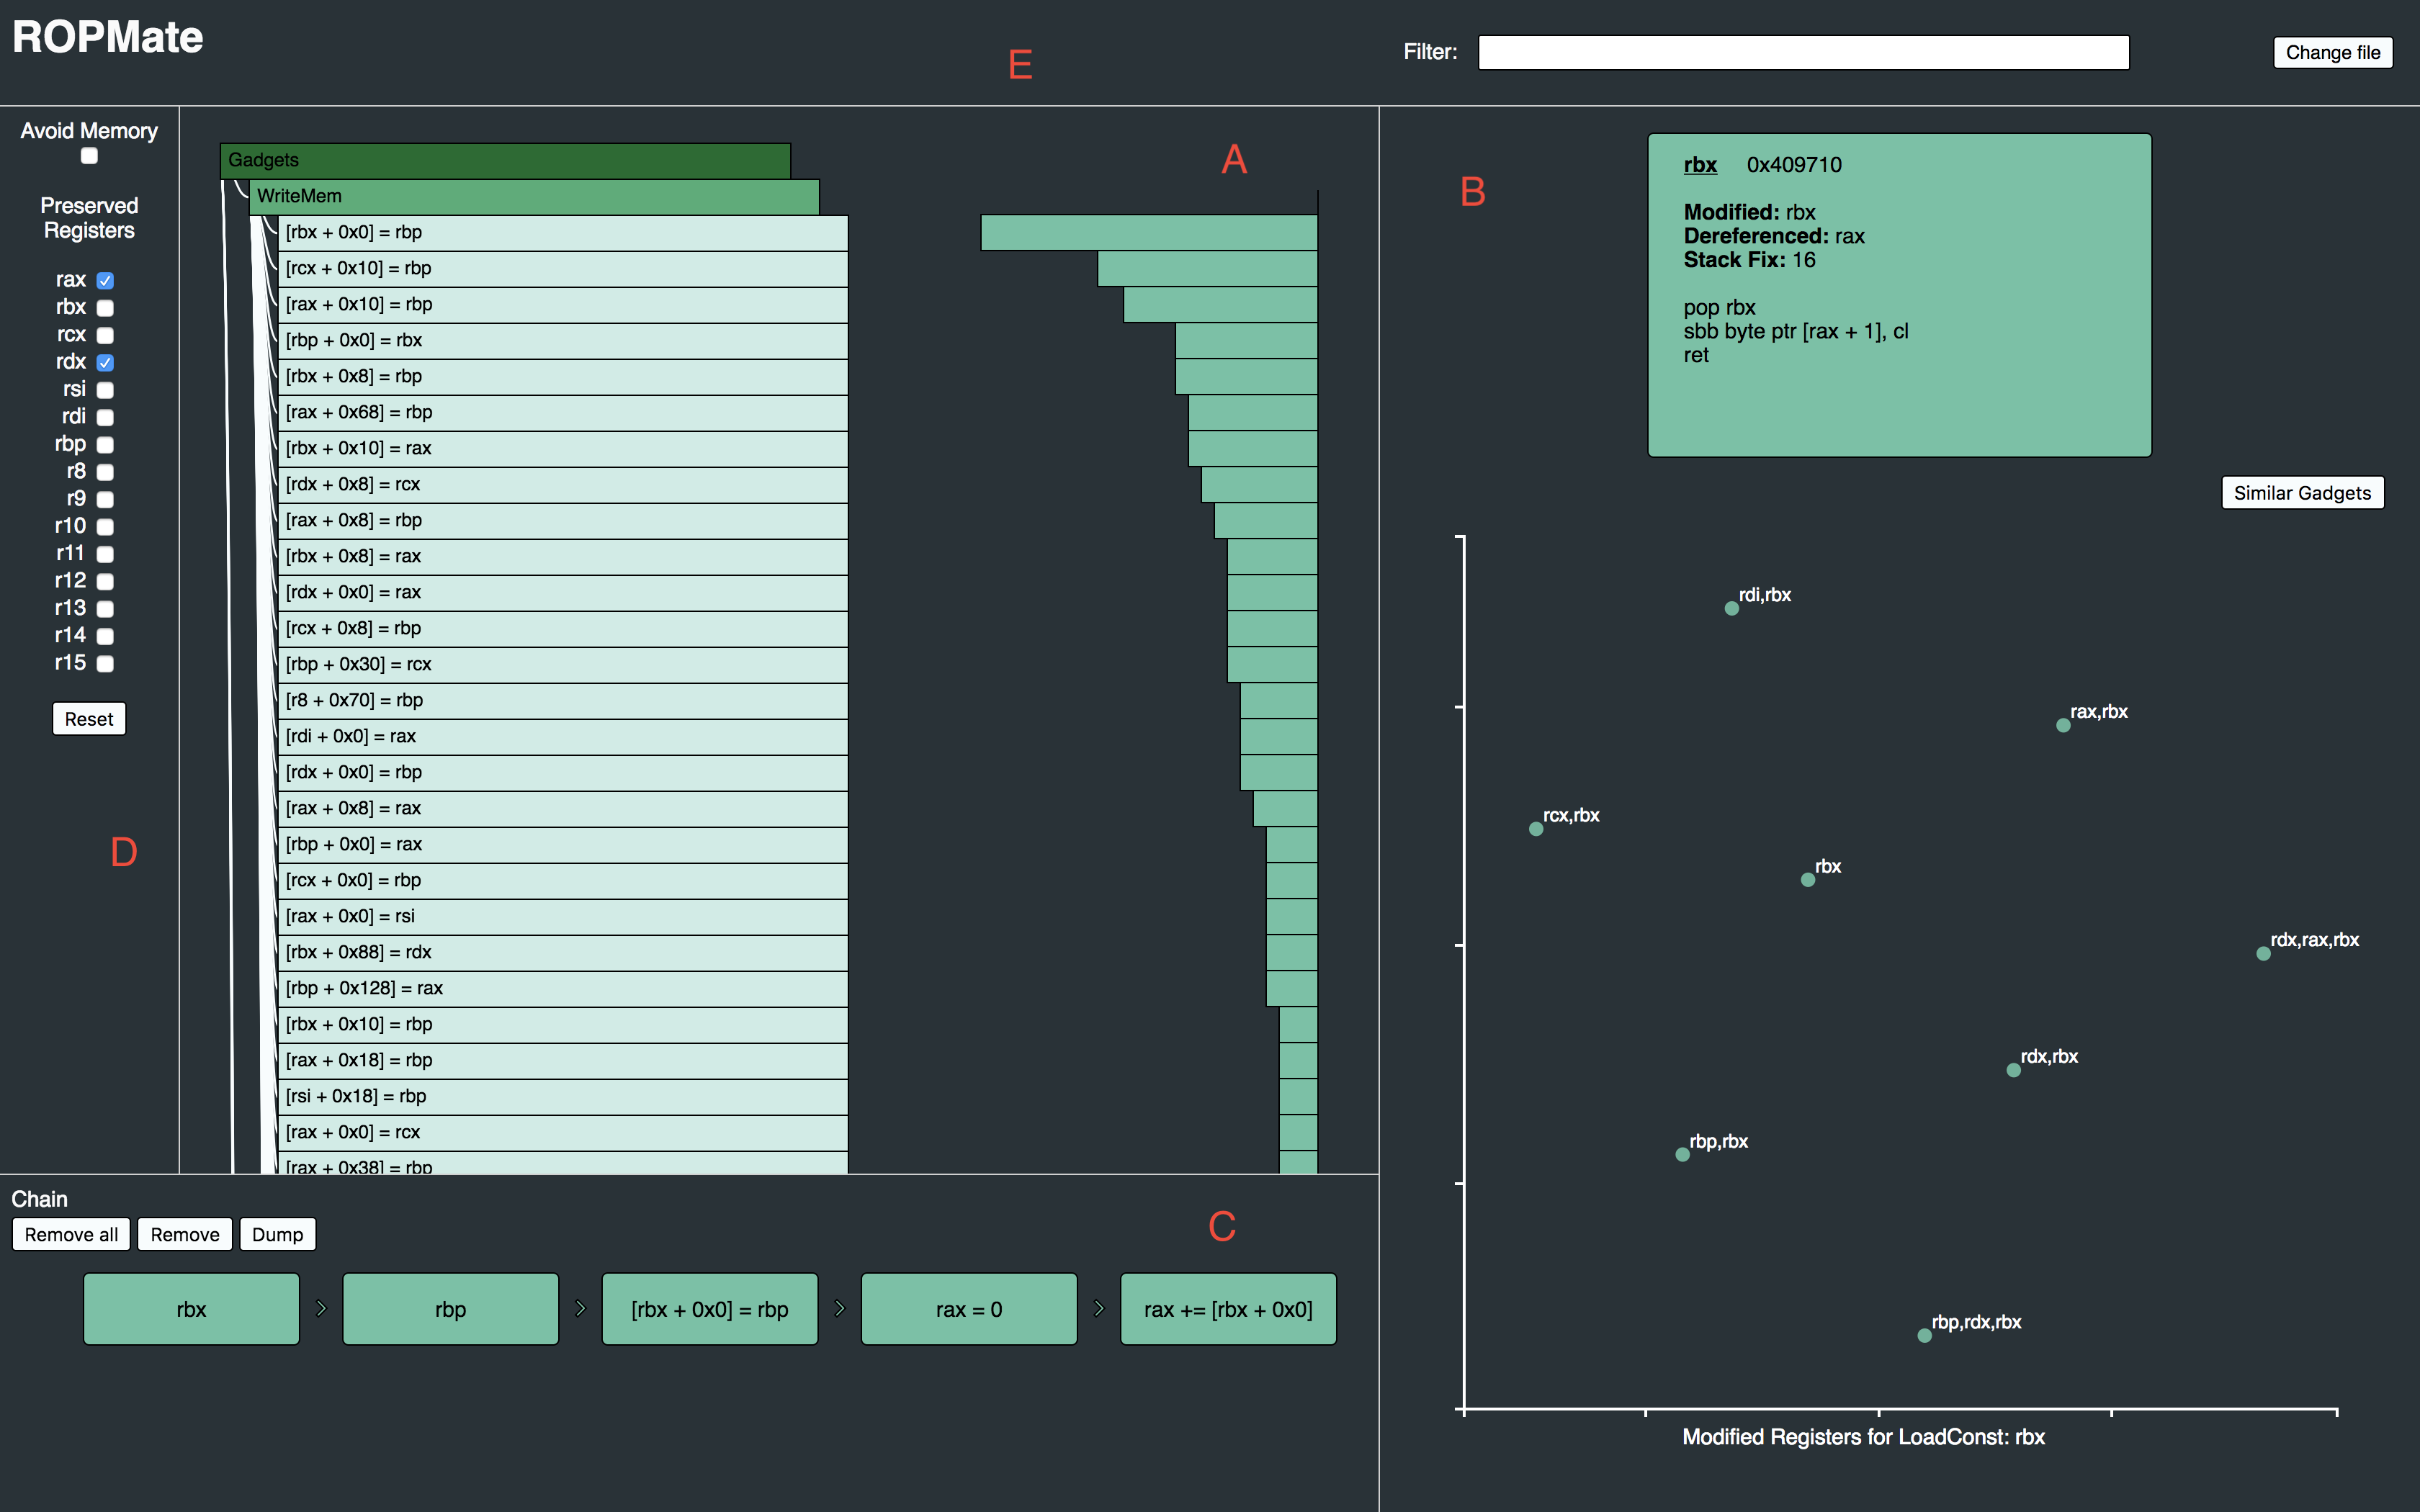
\includegraphics[width=0.9\linewidth]{ropmate-screen}
      \caption{ROPMate}\label{fig:ropmate}
    \end{figure}

\begin{abstract}

ROPChain based exploits are increasingly present in the scenario of advanced attack techniques.
Being able to test software against such types of attacks is fundamental to any RedTeam hacker. Automatic tool that try to create ROPChains exists and are well known, but they often fail with non usual binaries.
In this paper we propose \texttt{RopMate}, a visually aiding tool to help the human ROPChain builder to create its ROPChain. We strongly believe that there is the need of such a tool, since the existing state of the art only propose text based approach with, less or more, informative lists of the gadgets founded.
RopMate presents the builder with a clear interface of available gadgets, in which he is able to choose which of them to add to the building ROPChain, and, once selected, to filter the list according to wanted guarantees on preserved registers and accessed memory. The user is also able to find similar gadget in respect with the one chosen.
\end{abstract}

\twocolumn
\section{Introduction}
Return-oriented programming (ROP) is an exploiting technique that allows an attacker to induce arbitrary behavior in a vulnerable program without actually injecting any code, but through a chain of redirections in the program memory itself. \cite{rop}

The attack scenario is based on a controlled stack frame, where the return address can be overwritten. This is an advanced version of the ``return to libc attack'' \cite{libc} where multiple pieces of code are called in sequence to provide the needed code semantics execution: the attack combines a large number of short instruction sequences (called \textit{gadgets} from now on) that allow arbitrary computation. This is resilient to mitigation as non executable memory areas.

Each gadget is in the form of a couple of instruction followed by a return. This allows the attacker to place a sequence of gadget addresses on the stack (called \textit{ROPChain}) from the return address on, that will be executed thanks to the semantics of the ret instruction.

In this paper we aim to present a first step toward the acceptance that automatic tools will never be perfect, therefore human intervention will always be needed. Our tool is meant to give an help to any human ROPChain builder, in order to ease the creation of part or the totality of the chain.

While previous tools like, ropper \cite{ropper} or ROPGadget \cite{ROPGadget}, do an extraordinary job in finding useful gadgets, but they lack totally of user friendliness. They present the chain builder with a plain text dump of gadgets found, that is meant to be parsed by hand or scripting. While this is useful for other automatic tools, presenting the users with thousands of lines of gadgets doesn't help him in any way on the choice of the right gadget. Our work focuses on making the life of the exploiter easier.

\section{The Problem}
There exists automatic tools to find the suitable gadgets to create the final chain, but all of these tools present the attacker with a textual list of all the found gadgets. Then the attacker has to filter that list on the terminal with \texttt{grep} or similar commands. This becomes frustrating and infeasible with the growing of the complexity of the needed chain.

This is an example of the most simple ROPChain to spawn a shell in the libc standard library:

\begin{lstlisting}
rop = ''
rop += p64(...) # pop rdi; ret;
rop += '/bin/sh\x00'
rop += p64(...) # pop rsi; ret;
rop += p64(WRITABLE_ADDRESS)
rop += p64(...) # mov [rsi], rdi; ret;
rop += p64(...) # pop rdi; ret;
rop += p64(WRITABLE_ADDRESS)
rop += p64(...) # pop rsi; ret;
rop += p64(0x0)
rop += p64(...) # pop rax; ret;
rop += p64(...)
rop += p64(...) # syscall; ret;
\end{lstlisting}

\bigskip
Where \texttt{p64()} transforms an address to the string representation of it in 64 bits, to be able to place it on the stack:
\begin{lstlisting}
>>> p64(0x1122334455667788)
          '\x88\x77\x66\x55\x44\x33\x22\x11'
\end{lstlisting}

The comment near each instruction represents the instructions in that gadget to be executed.

\bigskip
The problem is that it never happens that the gadget are so simple and clear. Mixed with the instruction the attacker needs, there can be register modifications and memory accesses that can ruin the generated semantics, so choosing the next gadget to use is a delicate task. This becomes a pain, as the size of the chain grows and the number of constraints to maintain in mind increases.
Moreover the number of gadgets available in a binary is huge (from 1.500 for a middle sized binary to more than 15.000 for a standard library), so naively searching for useful and correct gadgets between them is impossible.

 Automatic tools that generate the chain exist but usually they fail and leave the attacker alone. So there is a lack of an effective tool to help developing the exploit.

\section{Related Works}
\label{se:related}
\paragraph{Code Reuse Attacks.}
Memory corruption bugs for memory unsafe languages are one of the oldest problems in software security. Historically, attackers have exploited buffer overflows caused by coding errors to inject their own code into the application and have the instruction pointer jump to it. Data Execution Prevention techniques, that are deployed on modern systems, try to mitigate execution of malicious payloads that can be inserted. Therefore Attackers have switched their attention to create attacks reusing code already present in the binary, calling functions present in the linked standard library or chaining together short instruction sequences to carry out the desired computation. Return Oriented Programming is the most famous embodiment of the latter approach: by arranging the addresses of the code sequences to be executed on the stack along with their operands as part of a ROP chain, the {\tt ret} instruction, present at the end of each gadget, instructs the CPU to follow the flow entailed by the chain.

\paragraph{ROP Gadget Finders.} There exists a plethora of tools to find executable gadgets (sequence of executable and correct instructions that ends with a {\tt ret} instruction): all of them provide the attacker with a list of gadgets among which to choose \cite{ropper} \cite{ROPGadget}.

\paragraph{Automatic ROPChain Builders.} Most of the tools, that provide some functionality to find gadgets, also try to automatically build a chain with some predefined desired effects. While they usually succeed with standard binaries (as {\tt libc}) or standard chains, they often fail on unusual binaries, and don't provide any help to build custom chains.

\paragraph{Visual ROPChain Builder.} At the time of the paper we weren't able to find any visual or textual tool, that would help an attacker to build his ROPChain. Current techniques just rely on python scripting.

\section{Proposed Solution}

We propose to apply Visual Analytics methods to the problem. The aim is to present an interface that will help the construction of the chain for the exploit.
The binary, that will be the source of the gadgets, is analyzed by the back-end server that produces a list of semantically meaningful gadgets. This means that only gadgets that have a clear effect are maintained.

The interface contains the list of all meaningful gadget, divided by class, and by effects on parameters, in which the user can make queries on the desired features and immediately visualize the gadgets that satisfy them.
Queries may involve searching for gadgets that have a particular semantical meaning, but for example, don't modify some registers that have yet been set or access the memory only by some controlled registers, not to crash the program.

Clicking on a gadget will show its features (that will be encoded with additional visual hints). Each class of gadget has a set of attributes listed in the Table~\ref{tab:gad_attr}.

\begin{table*}[htb]
\caption{Gadget attributes}\label{tab:gad_attr}
\centering
  \begin{tabular}{|l|l|}
    \hline
    \textbf{Gadget} & \\ \hline
    type & the class of the gadget \\ \hline
    params & the parameters of the gadget \\ \hline
    hex & the x86 bytes instructions in the gadgets \\ \hline
    disasm & the x86 disassembled instructions \\ \hline
    address & the address where the gadget starts in memory \\ \hline
    address\_end & the address where the gadget ends in memory \\ \hline
    modified\_regs & the registers modified by the execution of the gadget \\ \hline
    mem & the registers that the gadget uses to access memory \\ \hline
    stack\_fix & the delta in the stack after the gadget execution \\ \hline
    retn & how many words the ret instruction at the end pops out \\ \hline
  \end{tabular}
\end{table*}

\bigskip
Each gadget has a specific type, between:

\begin{center}
\noindent\texttt{LoadConst, SetZero, IncReg, CopyReg, }
\noindent\texttt{BinOp, ReadMem, WriteMem,}
\noindent\texttt{OpEsp, Lahf, ReadMemOp, WriteMemOp}
\end{center}

\section{ROPMate}
In this section we describe ROPMate, a prototype visual ROPChain builder, that assists the attacker in composing the chain with the desired semantics. ROPMate lets the user to filter and select gadgets to add to his chain, while presenting to him only the gadgets that fits the semantics and guarantees he wants. The user is also able to search for similar gadgets with respect to the selected one, needing the same semantics, but different guarantees.

\subsection{Gadgets Dataset} The system takes as input a dataset of semantically analyzed gadgets, provided by a back-end server. The back-end server essentially takes the original binary, collects the gadget through some existing gadget finding tool and performs a semantic analysis on each found gadget to set the type and the attributes described in Table~\ref{tab:gad_attr}.

\subsection{User Interface}
ROPMate is divided into five main views as shown in Figure~\ref{fig:ropmate}: the \textit{Tree View} (Figure~\ref{fig:ropmate}A), the \textit{Chain View}(Figure~\ref{fig:ropmate}C), the \textit{Analysis View}(Figure~\ref{fig:ropmate}B), the \textit{Control Panel} (Figure~\ref{fig:ropmate}D) and the \textit{Filter View} (Figure~\ref{fig:ropmate}E).

The user will search for the wanted gadget in the \textit{Tree View}, while inspecting the selected one and searching similar in the \textit{Analysis View}. Once added, a gadget, will show up in the \textit{Chain View}, and it can be further moved or removed from the chain. Filters in the \textit{Control Panel} and \textit{Filter View} can be user to restrict the search to useful gadgets.

\subsubsection{Tree View}
\begin{figure}[htb]
  \centering
  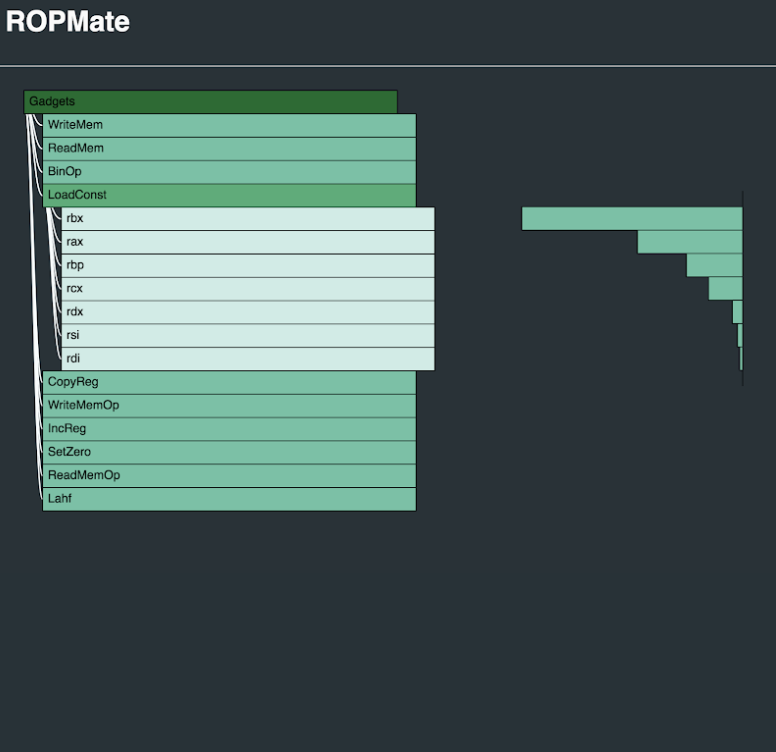
\includegraphics[width=0.6\linewidth]{tree-view}
\end{figure}

The \textit{Tree View} can be considered the main view of the tool: it provides the whole list of analyzed gadgets. Filters and controls apply to such list to restrict the search space. The gadgets in the main view are hierarchically ordered by class, and then by parameters that represents their semantic meaning (the list of categories reported in the previous section). In the last level of the tree the gadgets are presented displaying their assembly code. Since gadgets are aggregated by semantical meaning displaying the assembly code is the only way to distinguish them at first sight.

Near an opened category, an histogram is displayed, indicating to the user the number of gadgets of each class, to quickly give an hint on the overall view. Our first design choice was to integrate the histogram in the tree, but it lead to an ugly and unclear interface, therefore we chose to divide them.

\begin{figure}[htb]
  \centering
  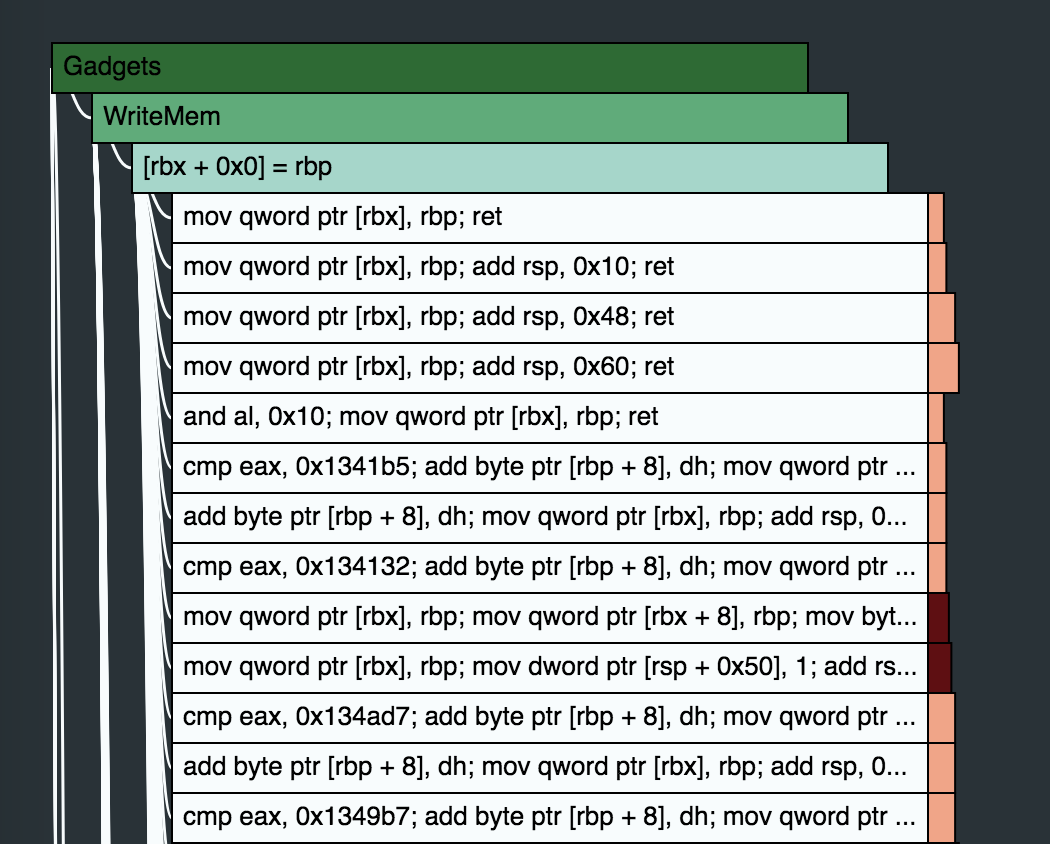
\includegraphics[width=0.8\linewidth]{tree-view_2}
\end{figure}

The last layer of the tree represents the gadgets. Each gadget is displayed in a line, and is coupled with a box on the side. The color of the box encodes the safety of the gadget with respect to memory, a lighter color indicates a low number of registers dereferenced to access memory, while a darker value encodes an high number, or an unknown access (on the stack but outside the gadget stack occupation). The length of the bar encodes the stack occupation of each gadget, therefore a longer bar will represent a gadget that needs more space on the stack.

Once the user selects a gadget, more information are displayed in the \textit{Analysis View}.

\subsubsection{Analysis View}
\begin{figure}[htb]
  \centering
  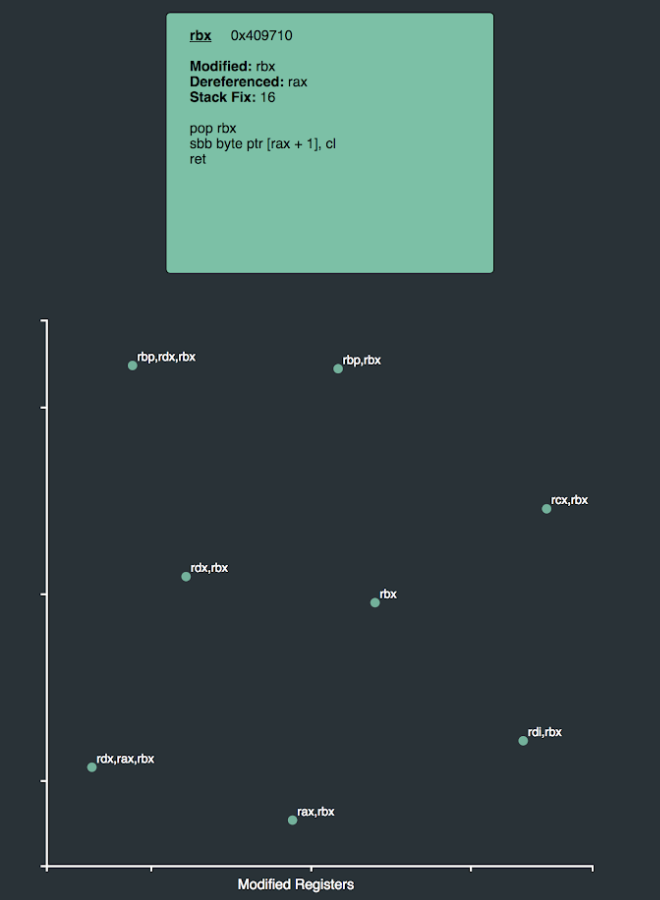
\includegraphics[width=0.6\linewidth]{analysis-view}
\end{figure}

The \textit{Analysis View} offers an insight of the selected gadget. It shows gadget attributes and offers the user the possibility to add the gadget to the chain or to search for similar gadgets. This is done by collecting all the gadget in the tree with the same semantics, and plotting them in a graph based their different modified register when executing. This allows the user to search for gadgets with the same effect, but that clobber different registers. Clicking on a displayed point will show the class of gadget in the \textit{Tree View} to visualize them.

The gadget placement in the scatterplot is based on Multidimensional Scaling where the dissimilarity function is simply the size of the modified registers that two gadgets have not in common. Therefore similar gadgets are displayed near each other, so that the user is able to quickly discriminate the possibilities from which it has to chose.

\subsubsection{Chain View}
\begin{figure}[htb]
  \centering
  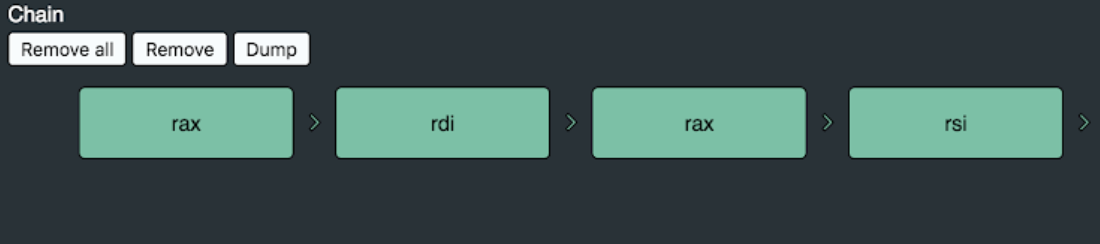
\includegraphics[width=0.7\linewidth]{chain-view}
\end{figure}

The \textit{Chain View} presents the current state of the built chain. Adding a gadget to the chain will trigger the recomputation for the registers the user has successfully set with the chain. By default, the view of the whole gadgets will display only the gadgets safe with respect to modified registers, that the user can choose.

It offers the possibility to move gadgets in the chain by dragging and dropping, and to remove them. Once the user is happy with the built chain clicking {\tt Dump} the system will generate a python script to integrate with current exploit technologies that will generate the byte-code of the chain, for example:

\begin{figure}[htb]
  \centering
  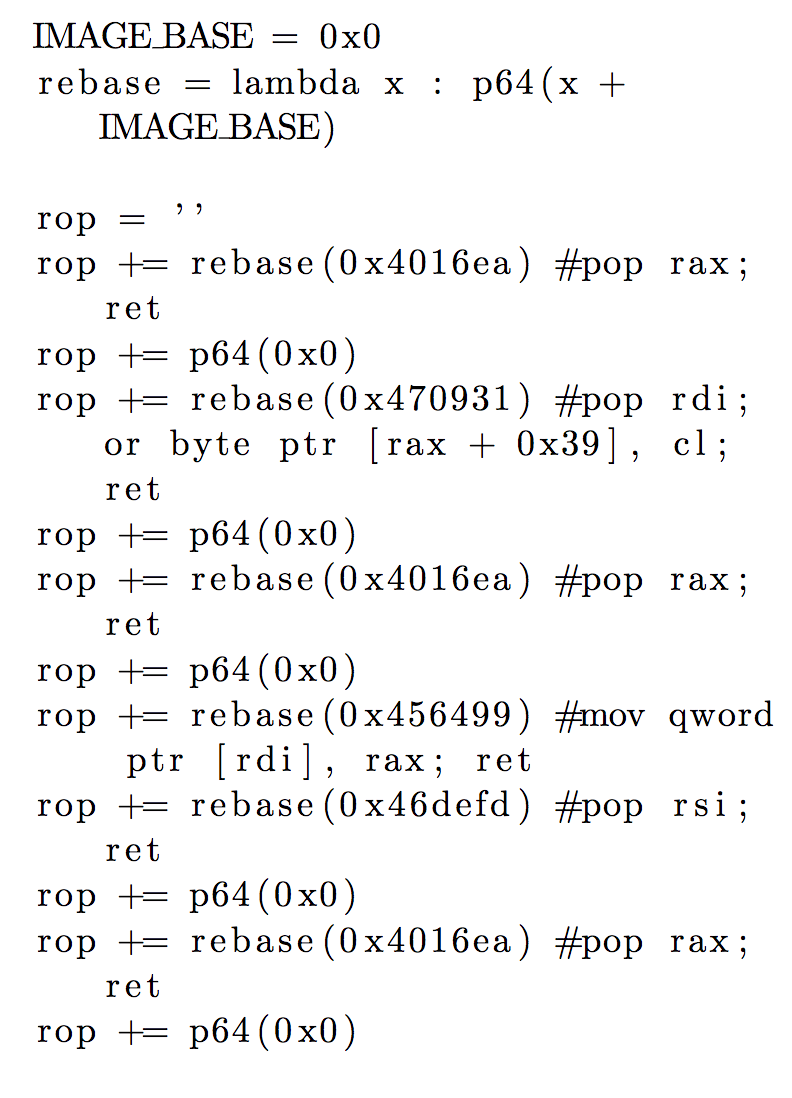
\includegraphics[width=0.8\linewidth]{dump}
\end{figure}

\subsubsection{Control Panel}
\begin{figure}[htb]
  \centering
  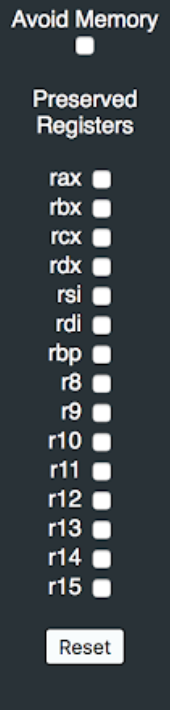
\includegraphics[width=0.15\linewidth]{control-panel}
\end{figure}

The \textit{Control Panel} allows the user to perform additional filtering on the gadget displayed. He is able to select which registers should be preserved in the gadget listing, to let the user safely choose gadget without clobbering registers set in the chain. The user has also the possibility to ask the system to display only gadgets that don't access memory (apart from the stack obviously) to be able to choose simpler gadgets first.

\subsubsection{Filter View}
\begin{figure}[htb]
  \centering
  
\includegraphics[width=0.8\linewidth]{filter-view}
\end{figure}

The \textit{Filter View}, jointly with the control panel, is used by the user to reduce the number of gadgets displayed, therefore to further simplify the research. The user is allowed to explicitly define the filter using a proper language. He is able to select all and only the gadgets that modify a particular register or have a given instruction.

\subsection{Finding Similar Gadgets}
The \textit{Similar Gadgets Finder} is triggered by the \texttt{Similar Gadgets} button in the \textit{Analysis View}. The module takes the \texttt{type} and \texttt{parameters} of the selected gadget to analyze only the semantically equivalent gadgets in the list. For each possible combination of gadgets it computes a dissimilarity function $f$. Where $f$ is:
$$
f(g_1, g_2) = |(M_1 \cup M_2) - (M_1 \cap M_2)|
$$
with $M_i$ being the set of modified registers by gadget $i$.

Then $MDS$ is applied to the dissimilarity matrix to compute a pair of coordinates for each gadget that will reflect the dissimilarity between gadgets in the relative distances. This shows the user a scatterplot in which similar gadgets are displayed near each other, allowing him to find semantically equivalent gadgets, but with different side effects. Figure~\ref{fig:mds} shows an example of the user searching different gadgets for the same semantical meaning (\texttt{[rbx] = rbp}).

\begin{figure}[htb]
\centering
 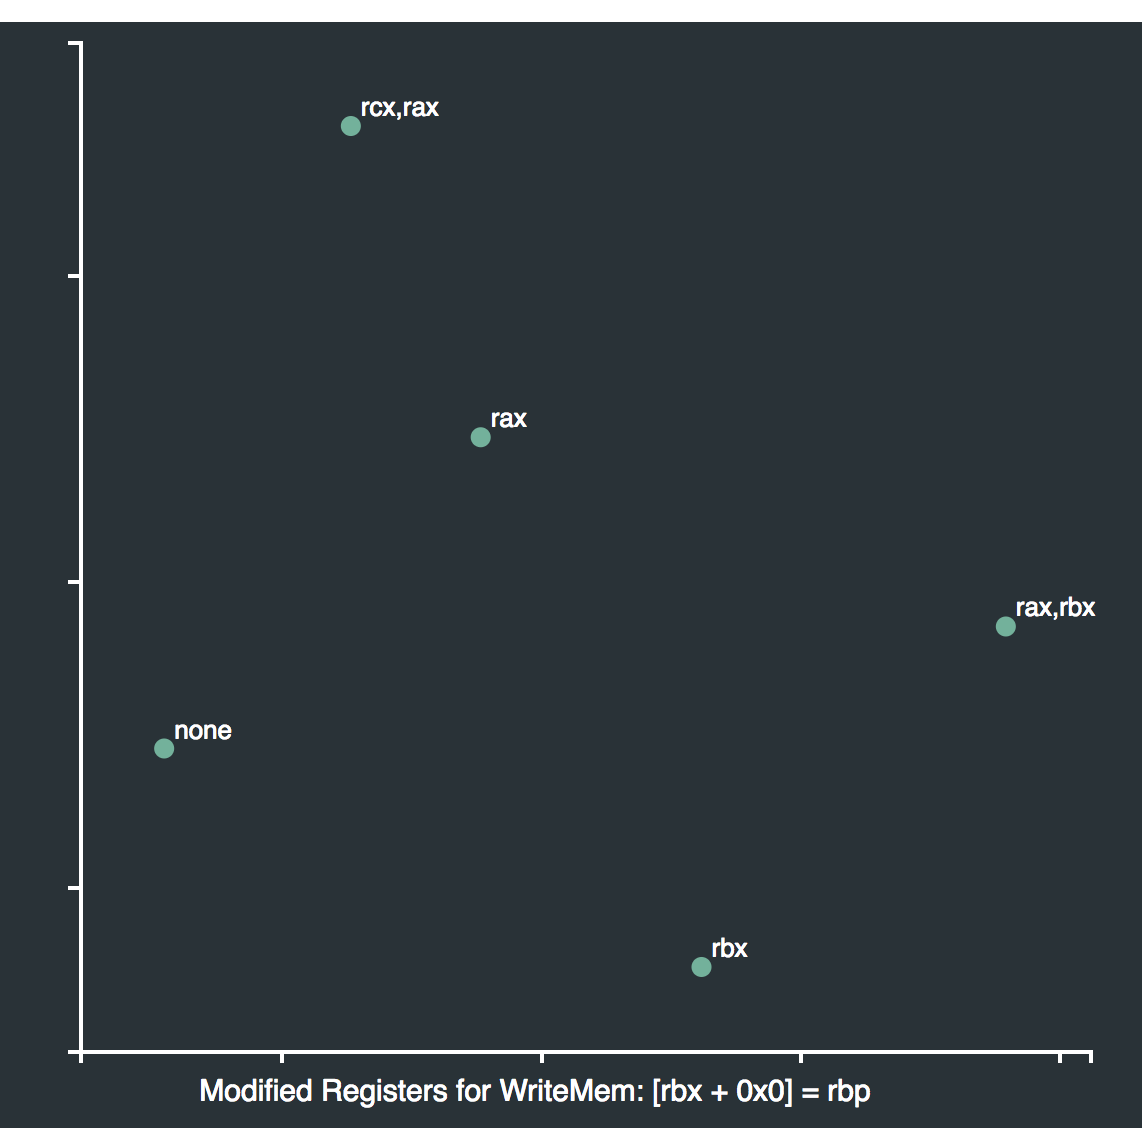
\includegraphics[width=0.4\textwidth]{mds}
 \caption{Similarity View}\label{fig:mds}
\end{figure}

It is important to note that it is possible that more than one gadget will have the same modified registers, therefore a single point in the scatterplot will possibly represent a set of gadgets. Clicking on the single point, the tree will display that set.

\section{User Evaluation}
It was conducted a session to gather preliminary user feedback from 4 participants that are experts in cyber security. The goal of the session was to obtain preliminary feedback on the general usability of the prototype system. Participants were first given a short description of how the prototype system works. They were then asked to use the prototype system and to think aloud throughout the entire session.

All participants believed the visual approach to the problem was very useful and user friendly. P2 and P3 observed that ROPMate acted as an interactive recommender for the next gadget to add to the chain. P4 commented that this approach to create the ROPChain allowed him to not be overwhelmed by useless gadgets. All participants thought that the interaction technique of clicking and filtering gadgets in the tree was easy to understand and found the classification helpful for searching efficiently the right gadget.

P1 and P2 appreciated that the histograms of the gadgets allowed them to have a visual representation of the number of registers modified and if the gadget access the memory or not. P3 expressed some frustration about about the dragging of gadgets in the presence of a long chain. P4 commented that it would have been nice to support advanced filters.

Given this preliminary feedback from users, we discuss the implications in greater detail in the next section.

\section{Limitations \& Future Works}
We present possible further work and open research challenges.

\textbf{Advanced filtering.} Although our prototype shows promising results for filtering the gadgets, we do not support complex filters, indeed the language to express the filter is quite limited.

\textbf{Select the gadget to remove.} When a new gadget is added to the chain, it is placed in the last position. We allow to delete this element or the entire chain through respectively the \textit{Remove} and the \textit{Remove all} button. The user can't delete any element of the chain. If he want to delete an element in the middle of the chain, he must drag it to the end of the chain and then click the \textit{Remove} button.

In a future work we can consider the possibility to select the gadget that the user wants to delete, so as to make the interaction more user friendly.

\textbf{Coordinate drag and scroll.} As evidenced by user experiences, if the chain becomes quite long, dragging the gadgets is difficult. The chain view does not move during the drag. So to drag a gadget in the presence of a long chain, the user must proceed by steps.

A possible solution, to be integrated in a future work, could be to synchronize drag of the gadget and scroll of the view.

\textbf{Insert guidance.} An interesting future work is to insert some guidance. A very useful guidance is to suggest to the user some combinations of gadgets to allow him to perform some specific operation that he had selected through the filter. This could allow the user to emulate the semantics of a single missing gadget, with the combination of some other. The additional chain would then be added to the built chain.

The guidance is not easy to implement because the system should analyze all the possible combinations of the gadgets. The problem would be exponential, therefore infeasible. Future work will involve designing some additional heuristics to cope with the problem.


\section{Conclusion}
Building a ROPChain is not an easy task. Understanding the semantics of each gadget, and finding the right one is increasingly difficult with the dimension of the set in which to choose. Current solutions support only the possibility to automatically build a chain and, if failed, they leave the attacker alone with a huge textual list of gadgets made by assembly instructions.
We presented \texttt{ROPMate} a prototype visual ROPChain builder, that assists the attacker in composing the chain with the desired semantics. Our tool makes the life of exploit creation easier, and assists the builder along the creation of the chain, proposing only gadgets with the desired guarantees and side effects. Additionally our tool finds similar gadgets with respect to user needs and shows them to the user.



\begin{thebibliography}{99}
  \bibitem{rop}
    Hovav Shacham,
    The Geometry of Innocent Flesh on the Bone: Return-into-libc without Function Calls (on the x86),
    CCS,
    2007.
  \bibitem{libc}
    Nergal,
    The advanced return-into-lib(c) exploits (PaX case study),
    Phrack Magazine 58(4),
    Dec. 2001.

    \bibitem{ropper}
     \url{https://github.com/sashs/Ropper},
    2018.

    \bibitem{ROPGadget}
    \url{https://github.com/JonathanSalwan/ROPgadget},
    2017.

\end{thebibliography}

\end{document}
